\documentclass[border=10pt]{standalone}
\usepackage{pgfplots}
\pgfplotsset{compat=1.17}

\begin{document}

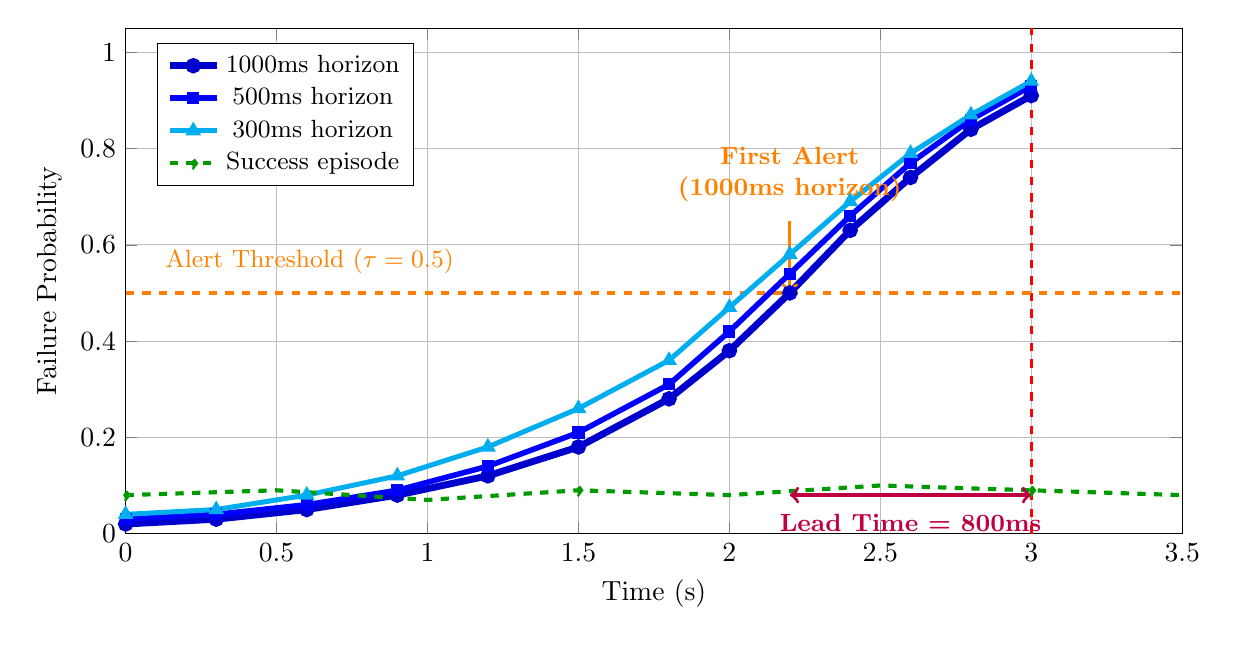
\begin{tikzpicture}
\begin{axis}[
    width=15cm,
    height=8cm,
    xlabel={Time (s)},
    ylabel={Failure Probability},
    legend pos=north west,
    grid=major,
    xmin=0, xmax=3.5,
    ymin=0, ymax=1.05,
    legend style={font=\small},
    every axis plot/.append style={thick}
]

% Ground truth failure at t=3.0s
\draw[red, very thick, dashed] (axis cs:3.0,0) -- (axis cs:3.0,1.05);
\node[anchor=south, color=red, font=\bfseries] at (axis cs:3.0,1.05) {Actual Failure};

% Alert threshold
\addplot[color=orange, dashed, line width=1.5pt, forget plot] coordinates {(0,0.5) (3.5,0.5)};
\node[anchor=south west, color=orange, font=\small] at (axis cs:0.1,0.52) {Alert Threshold ($\tau=0.5$)};

% 1000ms horizon prediction (dark blue)
\addplot[color=blue!80!black, line width=2.5pt, mark=*, mark size=1.5pt] coordinates {
    (0.0, 0.02) (0.3, 0.03) (0.6, 0.05) (0.9, 0.08)
    (1.2, 0.12) (1.5, 0.18) (1.8, 0.28) (2.0, 0.38)
    (2.2, 0.50) (2.4, 0.63) (2.6, 0.74) (2.8, 0.84)
    (3.0, 0.91)
};

% 500ms horizon prediction (blue)
\addplot[color=blue, line width=2pt, mark=square*, mark size=1.2pt] coordinates {
    (0.0, 0.03) (0.3, 0.04) (0.6, 0.06) (0.9, 0.09)
    (1.2, 0.14) (1.5, 0.21) (1.8, 0.31) (2.0, 0.42)
    (2.2, 0.54) (2.4, 0.66) (2.6, 0.77) (2.8, 0.86)
    (3.0, 0.93)
};

% 300ms horizon prediction (cyan)
\addplot[color=cyan, line width=1.8pt, mark=triangle*, mark size=1.5pt] coordinates {
    (0.0, 0.04) (0.3, 0.05) (0.6, 0.08) (0.9, 0.12)
    (1.2, 0.18) (1.5, 0.26) (1.8, 0.36) (2.0, 0.47)
    (2.2, 0.58) (2.4, 0.69) (2.6, 0.79) (2.8, 0.87)
    (3.0, 0.94)
};

% Success baseline (low probability)
\addplot[color=green!60!black, line width=1.5pt, dashed, mark=diamond*, mark size=1.2pt, mark repeat=3] coordinates {
    (0.0, 0.08) (0.5, 0.09) (1.0, 0.07) (1.5, 0.09)
    (2.0, 0.08) (2.5, 0.10) (3.0, 0.09) (3.5, 0.08)
};

% First alert annotation
\draw[orange, very thick, ->] (axis cs:2.2, 0.65) -- (axis cs:2.2, 0.50);
\node[anchor=south, color=orange, font=\small\bfseries, text width=3cm, align=center] at (axis cs:2.2, 0.67) {First Alert\\(1000ms horizon)};

% Lead time annotation
\draw[<->, very thick, color=purple] (axis cs:2.2, 0.08) -- (axis cs:3.0, 0.08);
\node[anchor=north, font=\small, color=purple] at (axis cs:2.6, 0.06) {\textbf{Lead Time = 800ms}};

\legend{1000ms horizon, 500ms horizon, 300ms horizon, Success episode}
\end{axis}
\end{tikzpicture}

\end{document}
